\documentclass{../Vorlage/mat}
\usetikzlibrary{shapes.misc}
\lstset{
	basicstyle=\small
}

\begin{document}
\maketitle{Sebastian Bliefert}{}{Nils Drebing}{}{Pascal Pieper}{}{15.12.2016}{Bonus} \\

\section*{Aufgabe A}
\begin{align*}
\phi & = 2 \pi \cdot \frac{47^{\circ}}{360^{\circ}}\\
& = 0.820304748437 
\end{align*}

\subsection*{a}
\begin{align*}
z & = exp(\imath \cdot \phi)\\
& = cos(\phi) + sin(\phi)i\\
& = cos(0.820304748437) + sin(0.820304748437)i\\
z & = 0.681998360062 + 0.731353701619i
\end{align*}
\newpage

\subsection*{b}
\begin{figure}[!htb]
\centering
	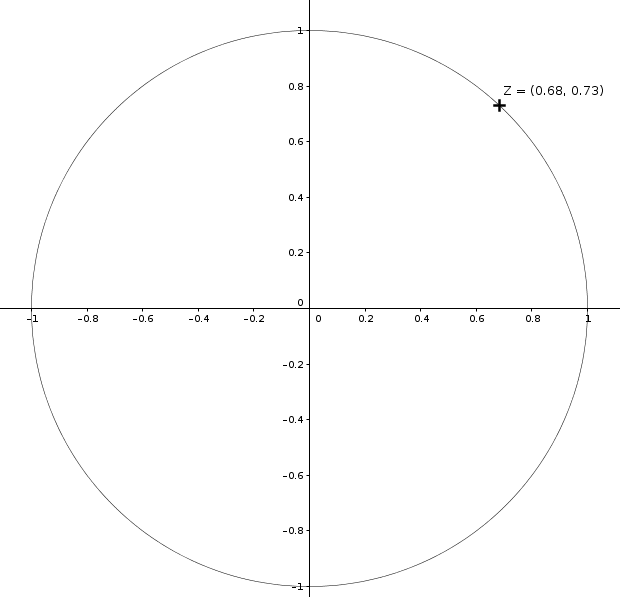
\includegraphics[scale=0.5]{circle_z.png}
	\label{circlez}
	\caption{Einheitskreis mit dem berechneten Punkt \textit{z}}
\end{figure}
\newpage

\subsection*{c}
\begin{figure}[!htb]
\centering
	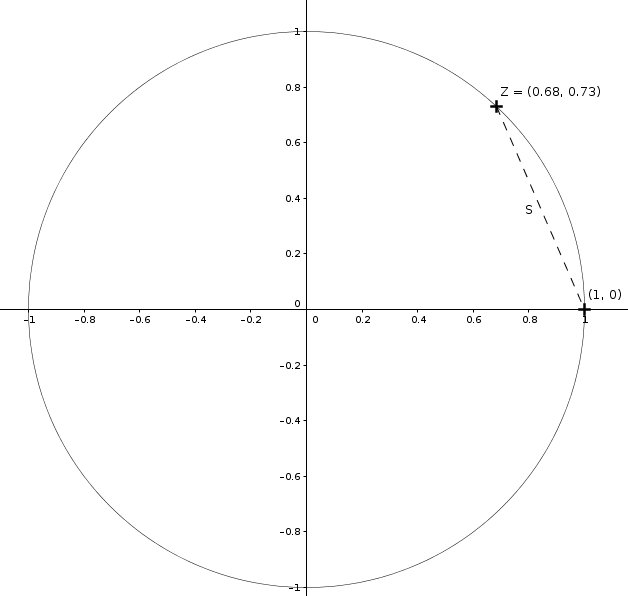
\includegraphics[scale=0.5]{circle_s.png}
	\label{circles}
	\caption{Einheitskreis mit dem berechneten Punkt \textit{z} und Strecke \textit{s} zwischen \textit{z} und $(1,0)^T$}
\end{figure}

\subsection*{d}
Nach Euklidischer Norm:
\begin{align*}
\|s\| & = \sqrt{(z_x - 1)^2 + (z_y - 0)^2}\\
& = \sqrt{(0.681998360062 - 1)^2 + 0.731353701619^2}\\
& = 0.79749813785
\end{align*}

\section*{Aufgabe B}

\section*{1.}
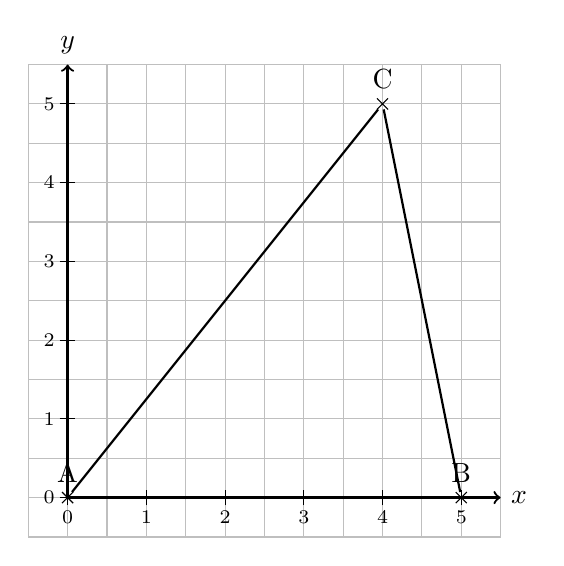
\begin{tikzpicture}[cross/.style={draw, cross out,
	minimum size=2*(#1-1pt), inner sep=0pt, outer sep=0pt}]
%Raster zeichnen
\draw [color=gray!50]  [step=5mm] (-.5,-.5) grid (5.5,5.5);
% Achsen zeichnen
\draw[->,thick] (0,0) -- (5.5,0) node[right] {$x$};
\draw[->,thick] (0,0) -- (0,5.5) node[above] {$y$};
% Achsen beschriften
\foreach \x in {0,1,2,3,4,5}
\draw (\x,-.1) -- (\x,.1) node[below=4pt] {$\scriptstyle\x$};
\foreach \y in {0,1,2,3,4,5}
\draw (-.1,\y) -- (.1,\y) node[left=4pt] {$\scriptstyle\y$};
%Punkte einzeichnen:
\node [cross=3pt,label={A},name=A] at (0,0) {};
\node [cross=3pt,label={B},name=B] at (5,0) {};
\node [cross=3pt,label={C},name=C] at (4,5) {};

\draw [thick, -] (A)--(B);
\draw [thick, -] (A)--(C);
\draw [thick, -] (B)--(C);

\end{tikzpicture}
\subsection*{2.}
\subsubsection*{Winkel bei A}
$$\overrightarrow{a_1}= \overrightarrow{AC}=C-A=\binom{4}{5} - \binom{0}{0} = \binom{4}{5}$$
$$|\overrightarrow{a_1}| = \sqrt{4^2+5^2} = \sqrt{41}$$
$$\overrightarrow{a_2} = \overrightarrow{AB} = B-A = \binom{5}{0} - \binom{0}{0} = \binom{5}{0}$$
$$|\overrightarrow{a_2}| =\sqrt{5^2+0^2} = \sqrt{25} = 5$$
$$ \cos{(\frac{\overrightarrow{a_1}\ast\overrightarrow{a_2}}{|\overrightarrow{a_1}|\cdot|\overrightarrow{a_2}|})} = \frac{4\cdot 5 + 5 \cdot 0}{\sqrt{41}\cdot 5} = \frac{20}{\sqrt{41}\cdot 5}$$
$$\alpha = \arccos{(\frac{20}{\sqrt{41}\cdot 5})} = 51^\circ = 2\pi\frac{51^\circ}{360^\circ} = 0,89 rad$$

\subsubsection*{Winkel bei B}
$$\overrightarrow{b_1}= \overrightarrow{BA}=A-B=\binom{0}{0} - \binom{5}{0} = \binom{-5}{0}$$
$$|\overrightarrow{b_1}| = \sqrt{(-5)^2+0^2} = \sqrt{25} = 5 $$
$$\overrightarrow{b_2} = \overrightarrow{BC} = C-B = \binom{4}{5} - \binom{5}{0} = \binom{-1}{5}$$
$$|\overrightarrow{b_2}| =\sqrt{(-1)^2+5^2} = \sqrt{26}$$
$$ \cos{(\frac{\overrightarrow{b_1}\ast\overrightarrow{b_2}}{|\overrightarrow{b_1}|\cdot|\overrightarrow{b_2}|})} = \frac{(-5)\cdot (-1) + 0 \cdot 5}{5\cdot \sqrt{26}} = \frac{5}{5\cdot\sqrt{26}}$$
$$\beta = \arccos{(\frac{5}{5\cdot\sqrt{26}})} = 79^\circ = 2\pi\frac{79^\circ}{360^\circ} = 1,38 rad$$

\subsubsection*{Winkel bei C}
$$\overrightarrow{c_1}= \overrightarrow{CB}=B-C=\binom{5}{0} - \binom{4}{5} = \binom{1}{-5}$$
$$|\overrightarrow{c_1}| = \sqrt{1^2+(-5)^2} = \sqrt{26}$$
$$\overrightarrow{c_2} = \overrightarrow{CA} = A-C = \binom{0}{0} - \binom{4}{5} = \binom{-4}{-5}$$
$$|\overrightarrow{c_2}| =\sqrt{(-4)^2+(-5)^2} = \sqrt{41}$$
$$ \cos{(\frac{\overrightarrow{c_1}\ast\overrightarrow{c_2}}{|\overrightarrow{c_1}|\cdot|\overrightarrow{c_2}|})} = \frac{1\cdot (-4) + (-5) \cdot (-5)}{\sqrt{26} \cdot \sqrt{41}} = \frac{21}{\sqrt{26} \cdot \sqrt{41}}$$
$$\gamma = \arccos{(\frac{21}{\sqrt{26} \cdot \sqrt{41}})} = 50^\circ = 2\pi\frac{50^\circ}{360^\circ} = 0,87 rad$$

\subsubsection*{Summe der Innenwinkel}
$$ \alpha + \beta + \gamma = 51^\circ+79^\circ+50^\circ = 180^\circ = \pi rad$$


\subsection*{3.}
$$ a = \overrightarrow{BC} = C-B = \binom{4}{5}-\binom{5}{0}= \binom{-1}{5} $$
$$ b = \overrightarrow{CA} = A-C = \binom{0}{0}-\binom{4}{5}= \binom{-4}{-5} $$
$$ c = \overrightarrow{AB} = B-A = \binom{5}{0}-\binom{0}{0}= \binom{5}{0} $$

\subsection*{4.}
Nothing


\section*{Aufgabe C}
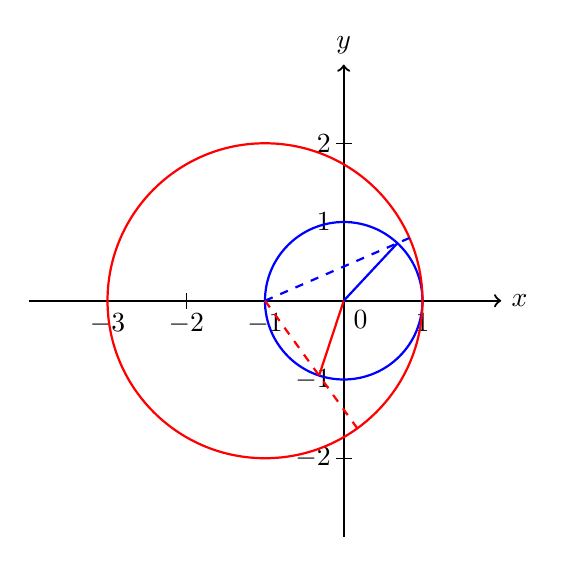
\begin{tikzpicture}
	\draw[->,thick] (-4,0) -- (2,0) node[right] {$x$};
	\draw[->,thick] (0,-3) -- (0,3) node[above] {$y$};
	
	\foreach \x in {-3,-2,-1,1}
	\draw (\x,-.1) -- (\x,.1) node[below=4pt] {$\x$};
	\foreach \y in {-2,-1,1,2}
	\draw (-.1,\y) -- (.1,\y) node[left=4pt] {$\y$};
	\draw (0,0) -- (0,0) node[below right] {$0$};
	
	%Aufgabe 2
	\draw[blue,thick] (0,0) circle [radius=1];
	\draw[red,thick] (-1,0) circle [radius=2];
	
	%Aufgabe 3
	\draw[blue,thick] (0,0) -- (0.682,0.731) node[] {};
	\draw[red,thick] (0,0) -- (-0.313,-0.950) node[] {};
	
	%Aufgabe 4
	\draw[blue,thick,dashed] (-1,0) -- (0.834,0.797) node[] {};
	\draw[red,thick,dashed] (-1,0) -- (0.172,-1.62) node[] {};
	
	
\end{tikzpicture}


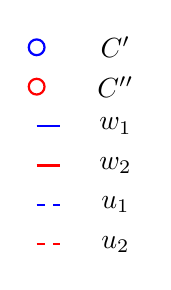
\begin{tikzpicture}
	\draw[blue,thick,circle] (0,0) circle [radius=0.1];
	\node at (1,0) {$C'$};
	\draw[red,thick,circle] (0,-0.5) circle [radius=0.1];
	\node at (1,-0.5) {$C''$};
	\draw[blue,thick] (0,-1) -- (0.3,-1);
	\node at (1,-1) {$w_1$};
	\draw[red,thick] (0,-1.5) -- (0.3,-1.5);
	\node at (1,-1.5) {$w_2$};
	\draw[blue,thick,dashed] (0,-2) -- (0.3,-2);
	\node at (1,-2) {$u_1$};
	\draw[red,thick,dashed] (0,-2.5) -- (0.3,-2.5);
	\node at (1,-2.5) {$u_2$};
\end{tikzpicture}


\subsection*{3}
$\phi_1 = 2 \pi \cdot \frac{47^\circ}{360^\circ} = 0,820$\\
$R_1 = 
\begin{bmatrix}
cos \phi_1 & -sin \phi_1\\
sin \phi_1 & cos \phi_1\\
\end{bmatrix}
=
\begin{bmatrix}
0,682 & -0,731\\
0,731 & 0,682\\
\end{bmatrix}$\\
$w_1 = R_1 \cdot v =
\begin{bmatrix}
0,682 & -0,731\\
0,731 & 0,682\\
\end{bmatrix}
\cdot
\begin{pmatrix}
1\\
0\\
\end{pmatrix}
=
\begin{pmatrix}
0,682\\
0,731\\
\end{pmatrix}
$\\
\\
$\phi_2 = 2 \pi \cdot \frac{-108^\circ}{360^\circ} = -1,889$\\
$R_2 = 
\begin{bmatrix}
cos \phi_2 & -sin \phi_2\\
sin \phi_2 & cos \phi_2\\
\end{bmatrix}
=
\begin{bmatrix}
-0,313 & 0,950\\
-0,950 & -0,313\\
\end{bmatrix}$\\
$w_2 = R_2 \cdot v =
\begin{bmatrix}
-0,313 & 0,950\\
-0,950 & -0,313\\
\end{bmatrix}
\cdot
\begin{pmatrix}
1\\
0\\
\end{pmatrix}
=
\begin{pmatrix}
-0,313\\
-0,950\\
\end{pmatrix}
$\\
\\
\subsection*{4}
$u'_1 = w_1 - c'' =
\begin{pmatrix}
0,682\\
0,731\\
\end{pmatrix}
-
\begin{pmatrix}
-1\\
0\\
\end{pmatrix}
=
\begin{pmatrix}
1,682\\
0,731\\
\end{pmatrix}$\\

$u_1 = \vec{u'}^0_1 \cdot 2 = 
\begin{pmatrix}
1,682\\
0,731\\
\end{pmatrix} / \sqrt{1,682^2+0,731^2} \cdot 2 = 
\begin{pmatrix}
1,834\\
0,797\\
\end{pmatrix}
$\\


$u'_2 = w_2 - c'' =
\begin{pmatrix}
-0,313\\
-0,950\\
\end{pmatrix}
-
\begin{pmatrix}
-1\\
0\\
\end{pmatrix}
=
\begin{pmatrix}
0,687\\
-0,950\\
\end{pmatrix}$\\

$u_2 = \vec{u'}^0_2 \cdot 2 = 
\begin{pmatrix}
0,687\\
-0,950\\
\end{pmatrix} / \sqrt{0,687^2+(-0,950)^2} \cdot 2 = 
\begin{pmatrix}
1,172\\
-1,620\\
\end{pmatrix}
$

\subsection*{5}
$ \varphi_1 = \mathtt{atan2}(0.797,1.834) = 0,410 = 23,488^\circ$\\
$ \varphi_2 = \mathtt{atan2}(-1.620,1.172) = -0,945 = -54,116^\circ$\\
\\
$ \frac{\varphi_1}{\phi_1} = \frac{0,410}{0,820} = 0.500$\\
$ \frac{\varphi_2}{\phi_2} = \frac{-0,945}{-1,889} = 0.500$

\subsection*{6}
$\mathtt{tan}(\phi_1/2) = 0.435$\\
$\mathtt{tan}(\phi_2/2) = 1.382$\\

Die Werte entsprechen den y Werten der beiden eingezeichneten, also um (-1,0) verschobenen, Vektoren $u_1$ und $u_2$ an ihrem jeweiligen Schnittpunkt mit der y-Achse.


\section*{Aufgabe D}
\subsection*{1}
\subsubsection*{(a)}
\begin{equation}
	R^{(1)} = \begin{pmatrix}
	0.87461971 & -0.4848092 & 0 \\
	0.4848092 & 0.87461971 & 0\\
	0&0&1
	\end{pmatrix}
\end{equation}
$q_0 = 1 + 0.87461971 + 0.87461971 + 1$\\
$q_1 = 0 - 0$\\
$q_2 = 0 - 0$\\
$q_3 = -0.4848092 - 0.4848092$\\
Also ist $\hat{q} = (3.74923942, 0, 0, 0.9696184)$
\subsubsection*{(b)}
$q_0 = \cos{\frac{\phi}{2}}$\\
$\mathbf{q} = \sin{\frac{\phi}{2}}\cdot j * \hat{n}$\\
\ldots magic \ldots\\
$\hat{n} = (0,0,0.25038)^T$\\
$\phi = 29\deg$
\subsection*{2}
\begin{align*}
\phi & = 2 \pi \cdot \frac{70^{\circ}}{360^{\circ}}\\
& = 0.820304748437 \\
\hat{n} & = (0,1,0)^T
\end{align*}
\subsubsection*{(a)}
\begin{align*}
R^{(2)} & = exp(\phi \cdot \hat{n}^\otimes) = I + sin(\phi) \cdot \hat{n}^\otimes + (1 - cos(\phi)) \cdot (\hat{n}^\otimes)^2\\
& = 
\begin{pmatrix}
1 & 0 & 0 \\
0 & 1 & 0\\
0 & 0 & 1 \\
\end{pmatrix} + sin(\phi) \cdot
\begin{pmatrix}
0 & 0 & 1 \\
0 & 0 & 0 \\
-1 & 0 & 0 \\
\end{pmatrix} + (1 - cos(\phi)) \cdot
\begin{pmatrix}
0 & 0 & 1 \\   
0 & 0 & 0 \\
-1 & 0 & 0 \\
\end{pmatrix}^2 						\\
& = 
\begin{pmatrix}
1 & 0 & 0 \\
0 & 1 & 0\\
0 & 0 & 1 \\
\end{pmatrix} +
\begin{pmatrix}
0 & 0 & 0.939 \\
0 & 0 & 0 \\
-0.939 & 0 & 0 \\
\end{pmatrix} + 
\begin{pmatrix}
0 & 0 & 0.658 \\   
0 & 0 & 0 \\
0.658 & 0 & 0 \\
\end{pmatrix} 						\\
R^{(2)} & =  
\begin{pmatrix}
1 & 0 & 1.5976 \\
0 & 1 & 0\\
-0.2817 & 0 & 1 \\
\end{pmatrix}
\end{align*}
%0.939 sin 
% 1 - cos phi = 0.657979856674
\subsubsection*{(b)}
\begin{align*}
\hat{q} & = cos(\frac{\phi}{2}) + sin(\frac{\phi}{2}) \cdot j * \hat{n}\\
& = 0.819152 + (0.573576j,0.573576k,0.573576l)^T * (0,1,0)^T\\
\hat{q} & = (0.819152, 0, 0.573576k, 0)
\end{align*}

\subsection*{3}
$R^{(3)} = \begin{pmatrix}
-1 & 0 & 0 \\
0 & 1 & 0\\
0 & 0 & -1\\
\end{pmatrix}
$\\
\textit{Rechenweg wie in Aufgabe 1}\\
$p = \left(0,0,2,0\right)$\\
$\hat{n} =(0,1,0) , \phi = 180\deg$


\subsection*{7}
\subsubsection*{(a)}
$R^{(1,3)} = \begin{pmatrix}
	-0.87461971 & -0.48480962 & -1.39729 \\
	-0.48480962 & 0.87461971 & -0.774532 \\
	0.2817 & 0 & -1 \\
	\end{pmatrix}$\\
$R^{(3,1)} = \begin{pmatrix}
	-0.87461971 & 0.48480962 & -1.5976\\
	0.48480962 & 0.87461971 & 0\\
	0.24638 & -0.136571 & -1\\
\end{pmatrix}$\\
$p_{(1,3)} = (0, -0.774532, 1.67899, 0)$\\
$\hat{n}_{(1,3)} = (-0.418886, 0.908039, 0) , \phi = 180\deg$\\

$p_{(3,1)} = (0, 0.136571, 1.84398, 0)$\\
$\hat{n}_{(3,1)} = (0.0738609, 0.997269, 0) , \phi = 180\deg$\\



	

\end{document}
